\section{Compilation Directives}
\label{sec:directives}

Since the introduction of heterogeneous parallel computing platforms tools have been developed to provide interfaces between compilers, runtimes and execution environments. The compilation directives is one of the approaches that has excelled in the context of parallel computing, because annotating code is usually easier than rewriting it. These directives are commonly implemented using the pre-processing directives \texttt{\#pragma}, in \texttt{C/C++}, and sentinels \texttt{!\$}, in the Fortran language.

Directives are used as annotations that provide tips about the original code and guide the compiler in the parallelization process of candidate regions. During the pre-processing, the \textit{tokens} that compose the directive can be replaced using macros, for example. The parallel version of the code will use features provided by the \texttt{OpenMP} runtime.

%\url{http://www.google.com/trends/explore#cat=0-5&q=openmp%2C%20hpf&cmpt=q&tz=Etc%2FGMT%2B3}
The use of directives was not introduced by \texttt{OpenMP}. Directives have been used as a macro specification language used in the pre-processing of languages such as C/C++ and Fortran. The macros transform the source code before the compilation. Languages such as \texttt{HPF} \cite{Richardson96highperformance} \cite{hpf:1997} had compiler directives for parallelism before the rise of \texttt{OpenMP}. However, with the popularity of multi-core processors and \texttt{OpenMP} supporting C/C++ and Fortran applications, \texttt{OpenMP} has become a robust runtime for multi-core processors and an interesting application of compilation directives. Figure~\ref{fig:google:trends:openmp} presents a comparison between the search results for the terms \lq\lq\texttt{OpenMP}\rq\rq{}, \lq\lq\texttt{HPF}\rq\rq{} (High Performance Fortran) and \lq\lq\texttt{Cilk}\rq\rq. The constantly higher number of searches for \lq\lq\texttt{OpenMP}\rq\rq{} can be taken as confirmation of its popularity.

\begin{figure}[htpb]
\centering
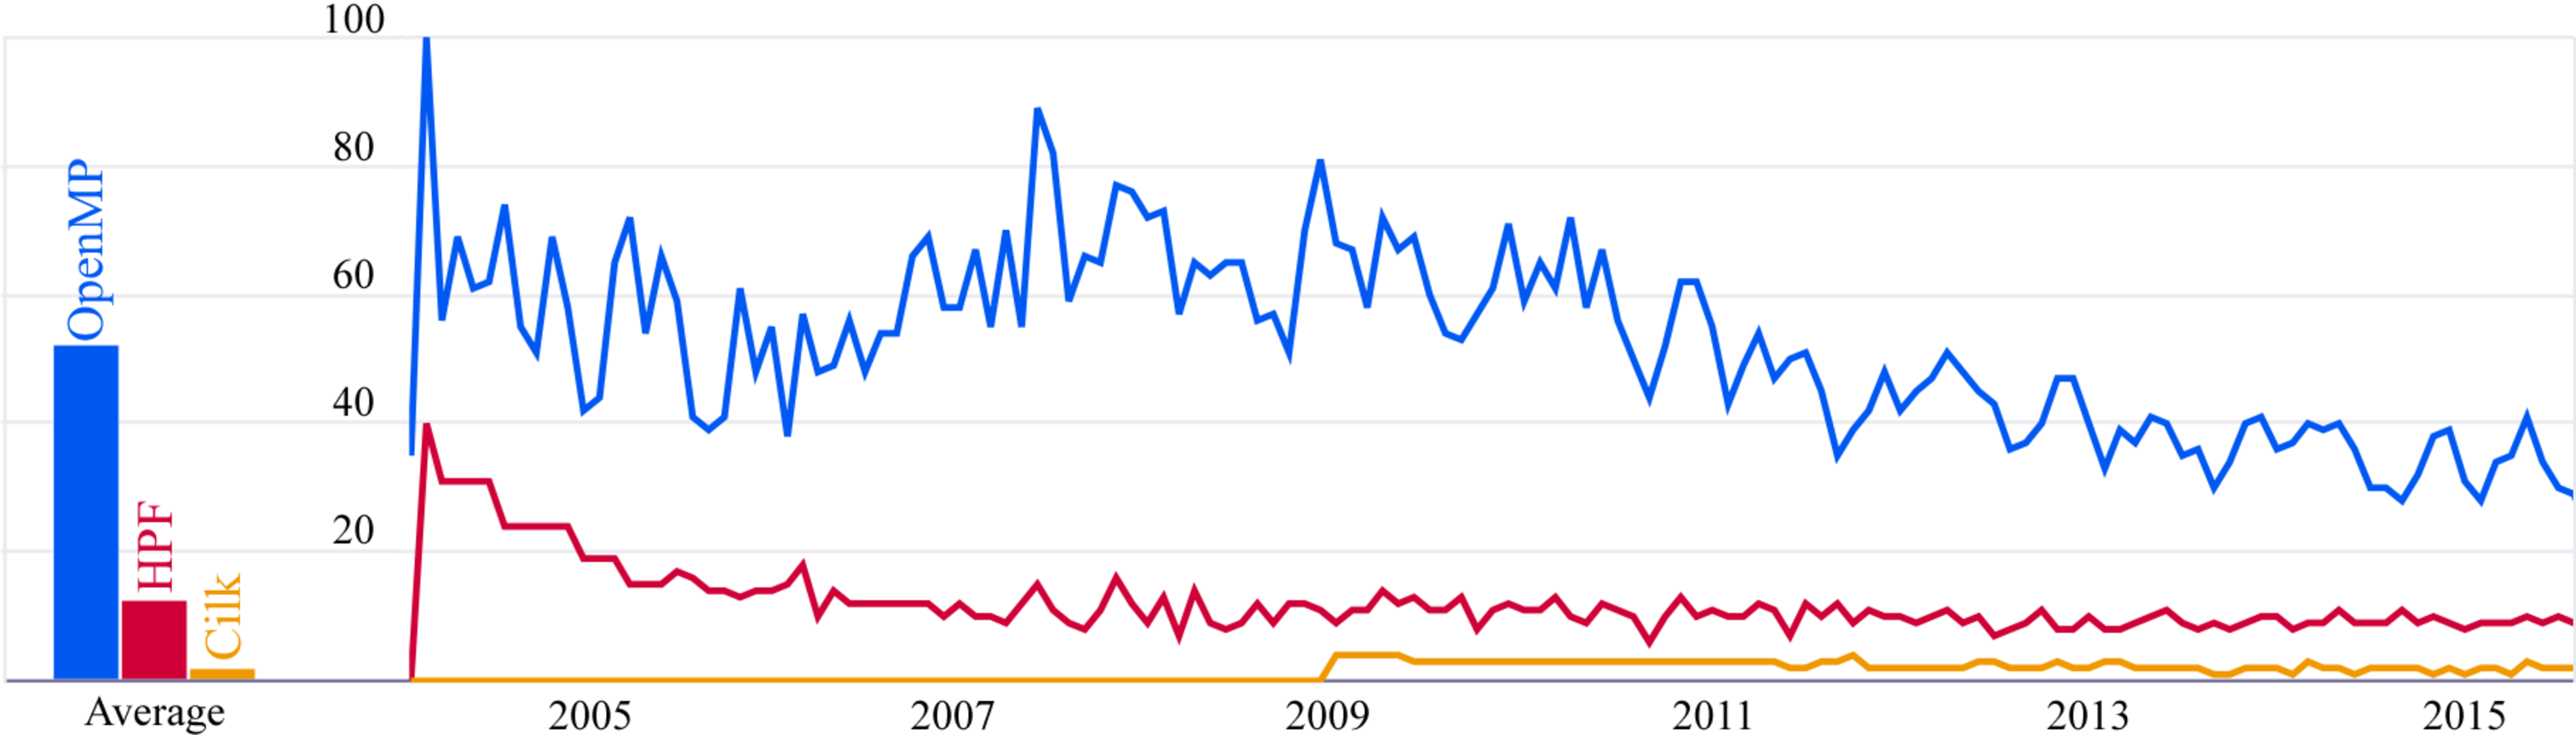
\includegraphics[width=1\columnwidth,height=0.35\columnwidth]{figures/google-trends-openmp.pdf}
\caption{Comparison of the Google Trends results for \lq\lq\texttt{OpenMP}\rq\rq, \lq\lq\texttt{HPF}\rq\rq{} and \lq\lq\texttt{Cilk}\rq\rq.}
\label{fig:google:trends:openmp}
\end{figure}

Using compilation directives is interesting because legacy code applications can be annotated and then parallelized by the runtime, to achieve performance improvements on multi-core processors. If the annotated code is analyzed by a compiler that supports \texttt{OpenMP} \cite{Dagum1998a} \cite{openmp:api:2011} \cite{openmp:api:2013} \cite{Chapman:2007} \cite{openmp:site}, a parallel version will be generated. Otherwise, the directives will be ignored and the code will remain sequential. Using the \texttt{OpenMP} runtime, parallel C/C++ or Fortran programming requires only the learning the directives' usage.

\texttt{OpenMP} is a set of compilation directives, functions libraries and environment variables that are based on the C/C++ and Fortran languages. The high level directives are able to expose the low level parallelism resources available on native implementations like the \texttt{pthreads} interface on GNU/Linux. Using the \texttt{OpenMP} directives much of the work is done automatically and implicitly, parallel regions have implicit barriers and the declaration of shared or private variables is simple.

\texttt{OpenMP} implements the \texttt{fork-join} model, in which multiple threads of execution perform tasks defined implicitly or explicitly by \texttt{OpenMP} directives~\cite{openmp:api:2011}~\cite{openmp:api:2013}. Threads are created from annotated code blocks. The \textit{master thread} executes sequentially until it finds the first parallel region. The similar \texttt{fork} operation creates a team of threads to execute a parallel region, the \textit{master thread} is part of the team. Nested parallel regions are allowed. When all threads in a team reach the barrier that marks the end of the parallel region, the master thread continues until it finds a new parallel region. From the annotated blocks, the runtime can generate implicit threads to execute the parallel regions or assign to some other thread the execution of explicit tasks defined by the programmer using the \texttt{task} directive.

Multiple compilers implement \texttt{OpenMP}, such as \texttt{GCC} \cite{libgomp:2015} and LLVM \texttt{clang} \cite{LLVM:CGO04} \cite{clang:site} \cite{openmp:llvm:site}, for example. \texttt{OpenMP} is certainly easier to use than \texttt{pthreads}~\cite{CPE:CPE529}. The directives allow a first contact with parallel programming that uses basic examples, letting the programmer experience an effortless application of parallel computing. However, complex parallel programming require more than simple \texttt{OpenMP} directives. Code~\ref{cod:sample:openmp} presents an example of the \texttt{OpenMP} compilation directives used to compute the dot product, which can be compared to a \texttt{pthreads} version presented in Code~\ref{cod:sample:vetdot:pthreads}.

\begin{lstlisting}[style=C, label=cod:sample:openmp,caption=Sample of OpenMP code.]
#pragma omp parallel firstprivate(aux_dot)
{
  #pragma omp single
  printf("Begin of the parallel region, number of threads: %d\n", omp_get_num_threads());
    
  #pragma omp for schedule(runtime)
  for(i = 0; i < SIZE; i++){ 
    aux_dot += A[i] * B[i];
  }
    
  #pragma omp critical
  dot += aux_dot;
    
  #pragma omp master
  printf("Final result: %d.\n", dot);
}
\end{lstlisting}

Expanding the code with directives allows to see how \texttt{OpenMP} reduces the amount of code that the programmer needs to write. The code with the expansions is shown in Code~\ref{cod:expanded:openmp}.

\begin{lstlisting}[style=C, label=cod:expanded:openmp,caption=OpenMP expanded code]
long long A[SIZE], B[SIZE], dot = 0;

void subfunction0 (void *data) {
  long long aux_dot = 0;
  
  if (GOMP_single_start ())
    printf("Begin of the parallel region, number of threads: %d\n", omp_get_num_threads());
  GOMP_barrier ();
  
  {
    long i, _s0, _e0;
    if (GOMP_loop_runtime_start (0, SIZE, 1, &_s0, &_e0))
      do {
        long _e1 = _e0;
        for (i = _s0; i < _e0; i++){
          aux_dot += A[i] * B[i];
        }
      } while (GOMP_loop_runtime_next (&_s0, &_e0));
    GOMP_loop_end ();
  }
  
  GOMP_critical_start();
  dot += aux_dot;
  GOMP_critical_end();
    
  if (omp_get_thread_num () == 0)
    printf("Final result: %d.\n", dot);
}

int main() {
  /* Initializations were supressed. */

  GOMP_parallel_start (subfunction0, NULL, 2);
  subfunction0 (NULL);
  GOMP_parallel_end ();

  return 0;
}
\end{lstlisting}

The Code~\ref{cod:expanded:openmp} shows calls to \texttt{GOMP\_parallel\_start()} \texttt{(line 33)} and \texttt{GOMP\_parallel\_end()} \texttt{(line 35)}. These functions are responsible to start and finish the team of threads that run \texttt{subfunction0(...)}. In the code it is also possible to see the functions that are mapped to barriers and synchronization. The calls to \texttt{GOMP\_barrier()} in \texttt{line 8}, \texttt{GOMP\_critical\_start()} and \texttt{GOMP\_critical\_end()} in \texttt{lines 22} and \texttt{24}, are mapped to semaphore and barrier primitives that are implemented in specific \texttt{OpenMP} libraries. 

The \texttt{OpenMP} runtime uses the standard thread library of the system, in this case, \texttt{pthreads}. The library is used together with other native system resources to control scheduling and synchronization. This shows that \texttt{OpenMP} is simpler comparing to code using \texttt{pthreads}, but the programmer still needs to master fundamental concepts about parallelism.

Tutorials present content in a structured way, showing the syntax of directives and exemplifying the use of annotations. The examples are simple in most cases, as can be seen in Code~\ref{cod:sample:openmp}. This kind of example brings to student the idea that \texttt{OpenMP} is always very simple. They simply annotate the code and make the program parallel.
In simple applications, we write one or two annotations in the code and generate a parallel version without difficulty. However, when we have more complex applications, it is necessary to know more concepts of parallel computing to apply the correct modifications in the source code. 

Another common situation when using compilation directives is obtaining a better performance for a parallel version of the code. It is necessary to perform large efforts to include the annotations and their proper restrictions. That turns the process into something like \lq\lq{}annotation or directive oriented programming\rq\rq. The time gained by not rewriting the application code is spent declaring directives and their restrictions.

Krawezik and Cappello~\cite{CPE:CPE905} evidenced this difficulty by comparing MPI and three OpenMP versions of benchmarks. The most popular use of \texttt{OpenMP} directives is at the loop level. In this approach the programmer discovers potentially parallel loops by profiling and checking the dependencies. The programmer then annotates the code with directives starting and closing parallel regions at each discovered parallelizable loop. However, good results were obtained only when SPMD was implemented on \texttt{OpenMP}, and achieving good performance required a significant programming effort~\cite{CPE:CPE905}.
